\chapter{Лічбавае асяродзьдзе}

\section{Жыцьцё анляйн}

Існуе толькі чатыры непасрэдныя прычыны сьмерці: спыненьне дыханьня, спыненьне сэрца, сьмерць мозгу і сыход у~інтэрнэт. Сапраўды, з~кожным годам мы праводзім усё больш часу ў~лічбавым асяродзьдзі, камунікуем там, працуем, вучымся, адпачываем і забаўляемся. Гэты трэнд будзе толькі ўзмацняцца ў~будучыні, таму мы ўпэўнена можам лічыць лічбавае асяродзьдзе часткай нашага навакольнага асяродзьдзя, а~значыць, яно ўплывае на стан здароўя чалавека гэтак жа актыўна, як і ўсё астатняе. Сіла і карысьць інфармацыйнага асяродзьдзя вельмі вялікія: мы можам працаваць з~дому, быць на сувязі, даведвацца пра навіны, мець доступ да сяброў і калег, абменьвацца ідэямі і весьці бізнэс. Чым хутчэй абменьваемся, чым вышэйшая шчыльнасьць ідэяў, тым мацней паскараецца разьвіцьцё. Інтэрнэт~--- гэта магутны інструмэнт, які паскарае тэмп нашага жыцьця, але можа паскорыць і выгараньне. Таму перад яго выкарыстаньнем (ці хаця б у~працэсе) важна вывучыць тэхніку бясьпекі.

\subsection*{Што мы робім анлайн}

\textbf{Уявім сабе двух людзей, якія па-рознаму выкарыстоўваюць лічбавыя тэхналёгіі.} Для аднаго чалавека яны~--- дадатковы навык, доступ да важнай інфармацыі, карысныя знаёмствы, кіраваньне рознымі праектамі адначасова. Пры гэтым ён не выкарыстоўвае інтэрнэт як замену рэальнага жыцьця, хутчэй, як яго працяг, узмацненьне, паскарэньне. Для іншага гэтыя ж тэхналёгіі могуць стаць крыніцай залежнасьці: ён пракрастынуе, скачучы па спасылках, ходзіць па чужых профілях, замяняючы гэтым рэальнае знаёмства, заліпае ў~сэрыялах і гульнях замест рэальных актыўных гульняў і адпачынку. Любая залежнасьць з~навакольнага сьвету можа быць памножаная і лёгка даступная ў~інтэрнэце: порна, казіно, гвалт, доступ да наркотыкаў.

Таму ў~гэтым разьдзеле я зьвяртаю больш увагі менавіта на патэнцыйна нэгатыўныя бакі, не прымяншаючы пры гэтым пераваг. Віртуальнае асяродзьдзе ўнікальнае~--- яно можа лёгка падладжвацца пад вас. У ім вы ўдзельнічаеце дыстанцыйна, практычна ананімна (умоўна, вядома), гэта дае пачуцьцё свабоды і зьмяншае адказнасьць, дазваляе стварыць сваю новую віртуальную асобу і паспрабаваць быць кім заўгодна.

Цяпер практычна палова насельніцтва сьвету карыстаецца сацыяльнымі сеткамі, праводзяць у~іх у~сярэднім дзьве гадзіны за дзень. А палова карыстальнікаў выкарыстоўвае некалькі розных сацыяльных сетак. Аднак смартфон~--- гэта ня толькі сацсеткі, але яшчэ і мноства праграмаў і гульняў. Таму ўласна ў~смартфоне людзі праводзяць яшчэ больш часу~--- да пяці гадзінаў на содні, з~іх 26\,\%~--- каля сямі гадзінаў. Гэта вялікая колькасьць часу, бо за месяц ``невялікія'' 2,5 гадзіны ў~дзень ператвараюцца ў~тры дні, а~за год~--- больш чым у~месяц.

Выкарыстоўваючы лічбавае асяродзьдзе для вырашэньня канкрэтных задач, факусуючыся на мэце, мы атрымліваем карысьць. Але калі мы выкарыстоўваем смартфоны пасіўна, для забаўкі ці адцягненьня, тады наша ўвага кіруецца вонкавымі алгарытмамі, а~ня ўласнымі мэтамі, а~гэта можа быць небясьпечна для здароўя. Такое спажываньне лічбавага кантэнту можна параўнаць са спажываньнем фастфуду.

\emph{Мне падабаецца параўноўваць харчаваньне і інфармацыю, падрабязна разьвіў гэтую тэму Фрэдэрык Пэрлз у~«Эга, голад і агрэсія». Гэтая мэтафара можа быць нам карысная, бо яна дастаткова дакладна дапамагае зразумець і сфармуляваць працэс узаемадзеяньня нашага мозгу ў~інфармацыйным асяродзьдзі.} 

Памятаеце, да інтэрнэту мы думалі, што прычына дурных паводзінаў~--- гэта недахоп інфармацыі? Як жа мы памыляліся! Багацьце інфармацыі не заўсёды добрае. Бо наш мозг схільны выбіраць найлягчэйшыя рашэньні: як у~харчаваньні нас цягне на самыя калярыйныя з~прадуктаў: цукар, тлушч і іх спалучэньні,~--- так нас аўтаматычна прыцягвае ўся інфармацыя, што закранае эмоцыі, выклікае цікаўнасьць і страх.

\textbf{Інфармацыйны фастфуд} дробніцца на невялікія порцыі, у~выглядзе цукерак або батонікаў, мы ў~прамым сэнсе ``перакусваем'' інфармацыяй для ўзьняцьця настрою. А гэта можа прывесьці да неспрыяльных наступстваў. Навукоўцы ўсталявалі, што бессэнсоўны сэрфінг у~інтэрнэце можа быць справакаваны бязьдзеяньнем, неабходнасьцю адпачынку ад нуднай працы, пазьбяганьнем сацыяльнага ўзаемадзеяньня або неабходнасьцю чаканьня званка ці паведамленьня.

\emph{«Чалавечае шчасьце сёньня ў~тым, каб забаўляцца. Забаўляцца~--- гэта значыць атрымліваць задавальненьне ад ужываньня тавараў, відовішчаў, ежы, напояў, цыгарэтаў, людзей, лекцыяў, кніг, кінакарцін~--- усё спажываецца, паглынаецца. Сьвет~--- гэта адзін вялікі прадмет нашага апэтыту, вялікі яблык, вялікая бутэлька, вялікія грудзі; мы~--- смактункі, вечна чагосьці чакаем, вечна на нешта спадзяваемся~--- і вечна расчараваныя». Эрых Фром.} 

Зразумела, ня варта дэманізаваць смартфоны, як і праклінаць гамбургеры з~малочнымі кактэйлямі. Смартфон~--- гэта самая важная рэч з~тых, што заўсёды з~намі, і ён сапраўды добра дапамагае. Як правіла, размовы аб тым, што смартфон робіць нас тупымі~--- гэта перабольшаньне, аднак шэраг важных заўваг усё ж такі ёсьць. Цяпер мы ня можам сказаць, колькі часу~--- норма, а~колькі~--- ужо залежнасьць, але калі ёсьць зьніжэньне якасьці жыцьця праз злоўжываньне смартфонам, то ёсьць і праблема.

\begin{figure}[htb!]
  \centering
  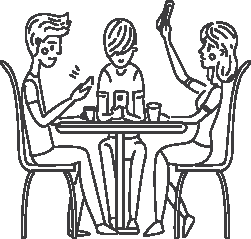
\includegraphics[scale=1.5]{willpower/ch13/1.pdf}
\end{figure}

\subsection*{Пабочныя эфэкты}

Яны ёсьць заўсёды і ад усяго. Таму, як і з~харчаваньнем, трэба адсочваць свой рэжым і рацыён узаемадзеяньня са смартфонам. Замест вядзеньня харчовага дзёньніка дастаткова ўсталяваць праграмы (Quality Time BreakFree, Moment для iOS і інш.), якія адзначаюць, колькі разоў вы карыстаецеся тэлефонам і сумарны час выкарыстаньня, а~ў сваім дзёньніку адзначайце ваша самаадчуваньне.

\infobox{У смартфоне важна цалкам адключыць усе апавяшчэньням~--- банэры і гукі,~--- акрамя крытычна важных.}

Калі ў~вас больш за 80\,\% цэльнай якаснай ежы, то вы можаце дазволіць сабе адступленьні. Тое ж самае з~тэлефонам~--- ён небясьпечны, калі яго занадта шмат. Дасьледаваньні паказваюць, што 47\,\% амерыканцаў сьвядома прыкладаюць намаганьні, каб абмежаваць яго выкарыстаньне.

\emph{Падобная сытуацыя з~працай мозгу і некаторымі кагнітыўнымі навыкамі~--- яны паляпшаюцца, калі не адцягвацца, і вінаваты тут ня толькі смартфон. Прадукцыйнасьць працы без тэлефона паляпшаецца на 26\,\%, расьце і пасьпяховасьць школьнікаў.}

Калі мы выкарыстоўваем смартфоны бескантрольна, яны могуць, як і пераяданьне, сапсаваць наш мозг, зрабіць яго больш ``тлустым'' і ``лянівым''. Кантралюйце гэты працэс, вылучайце, як і ў~харчаваньні, ``чыстыя прамежкі'' для творчасьці і камунікацыі. Калі для цела існуе спорт, каб выдаткаваць калёрыі, то для мозгу існуе крэатыў~--- прыдумляйце новае кожны дзень, стварайце і практыкуйце свой мозг.

\subsection*{Пытаньні і заданьні}

1. Вы карыстаецеся інтэрнэтам ці інтэрнэт выкарыстоўвае вас?

2. Ці ёсьць у~вас мяжа паміж збалянсаваным спажываньнем інфармацыі і яе лішкам?

3. Ці адчуваеце вы перагрузку інфармацыяй?


\section{Уплыў на здароўе}

Азірніцеся вакол~--- і вы ўбачыце, што шматлікія людзі праводзяць час ня столькі ўдома ці на працы, а~менавіта ў~лічбавым асяродзьдзі: ад 4 да 16 гадзінаў на дзень~--- гэта вельмі шмат. Чым больш мы там, тым менш у~нас застаецца часу для камунікацыі, руху, спорту, падарожжаў, прыродаў і да т.~п.

\emph{Інтэрнэт моцна ўплывае на маю нэрвовую сыстэму: я пачынаю шалёна злавацца, калі ён павольны ці зьнікае!}

Смартфон уплывае на нас, нават калі мы ім не карыстаемся. Навукоўцы ўсталявалі, што проста фізычная прысутнасьць тэлефона побач пагаршае нашу ўвагу і зьніжае кагнітыўныя здольнасьці. Смарфтон не расслабляе, у~дасьледаваньнях тыя людзі, хто падчас перапынку ``сядзеў у~тэлефоне'', на 22\,\% горш спраўляліся з~тэстамі, чым тыя, хто проста адпачываў.

Дасьледаваньні на МРТ паказваюць, што ў~людзей з~залежнасьцю ад тэлефона ёсьць такія ж зьмены ў~мозгу, як пры іншых залежнасьцях: зьніжаецца колькасьць шэрага рэчыва ў~скроневай кары, астраўковай долі, падае актыўнасьць пярэдняй зьвіліны поясу, якая адказвае за кантроль эмоцыяў, прыняцьце рашэньняў. Умоўна можна вылучыць некалькі тыпаў нэгатыўнага ўзьдзеяньня.

\subsection*{Залежнасьць}

Многія дасьледчыкі ўпэўненыя, што залежнасьць ад смартфона можна паставіць у~адзін шэраг з~такімі нехімічнымі залежнасьцямі, як шопінг, гемблінг і да т.~п. Рызыка стаць залежным вышэй у~тых людзей, у~каго ўжо ёсьць існыя залежнасьці і схільнасьць да імпульсіўных паводзінаў.

\textbf{Звычайна залежнасьць праяўляецца ў~не\-маг\-чы\-масьці засяродзіцца і сындроме адмены, калі чалавек без тэлефона становіцца раздражнёным і адчувае сябе вельмі дыскамфортна. Да 70\,\% амерыканцаў ня могуць заснуць без свайго тэлефона.} 

Людзі імкнуцца ня толькі лёгка атрымаць задавальненьне, але й лёгка пазбавіцца непрыемных пачуцьцяў без намаганьняў. Таму мы даём нырца ў~тэлефон, замест таго каб разабрацца, чаму нам кепска.

\textbf{Крытэрыі любой залежнасьці досыць простыя:} 
\begin{itemize}
  \item \textbf{прывыканьне}: зь цягам часу вам трэба больш часу для атрыманьня такога ж эфэкту;
  \item \textbf{адвыканьне}: нэгатыўныя адчуваньні пры спыненьні выкарыстаньня тэлефона і сацсетак;
  \item \textbf{злоўжываньне}: калі вы хочаце правесьці ў~інстаграме 20 хвілінаў, а~праводзіце гадзіну;
  \item \textbf{страта кантролю}: вашы паводзіны мяняюцца, вам цяжка кантраляваць і абмяжоўваць сябе;
  \item \textbf{выключныя намаганьні для атрыманьня}: калі вы стараецеся быць анляйн ня толькі дома ці на працы, але й па дарозе, на хаду;
  \item \textbf{празьмерная прыярытэзацыя}: калі вы седзіце ў~інтэрнэце на шкоду вашым асноўным справам, працы, сям'і і да т.~п.
\end{itemize}

\begin{figure}[htb!]
  \centering
  
\includegraphics[scale=1.5]{willpower/ch13/2.pdf}
\end{figure}

Вялікая колькасьць праведзенага ў~фэйсбуку, інстраграме і твітары часу была зьвязаная з~сымптомамі дэпрэсіі: страта задавальненьня, пачуцьцё безнадзейнасьці, віны і да т.~п. Узаемасувязь паміж выкарыстаньнем смартфона і дэпрэсіяй дастаткова складаная, наўрад ці менавіта тэлефон выклікае дэпрэсію, а~вось дэпрэсія, як правіла, можа выяўляцца павелічэньнем працягласьці часу выкарыстаньня смартфона.

\textbf{З розных відаў лічбавай актыўнасьці толькі сацыяльныя сеткі і тэлевізар карэлююць з~рызыкай дэпрэсіі, а~вось звычайны інтэрнэт-сэрфінг і відэагульні ніяк з~дэпрэсіяй не зьвязаныя.}

\textbf{Дзеці і тэлефоны.} Многія бацькі выкарыстоўваюць тэлефоны як соску, каб ``заткнуць'' або заняць дзіця. Цяпер дзеці ва ўзросьце 10 гадоў і раней маюць уласны тэлефон і праводзяць там 4--5 гадзінаў штодзень. Бацькі таксама ўсё менш займаюцца зь дзецьмі, а~нават у~астатнія гадзіны яны ня могуць даць ім увагі, самі ўвесь час адцягваючыся на тэлефон. Тым ня менш малодшае пакаленьне хутка адаптуецца, таму дзеці могуць нават анляйн заводзіць глыбокія сацыяльныя сувязі, замацоўваць адносіны зь сябрамі, напрыклад, падчас сумеснай анляйн-гульні. Апошнім часам радыус прасторы, у~якім дзеці дасьледуюць сьвет, скараціўся на 90\,\%!

\textbf{Віртуальнае ці жывое.} Шэраг дасьледаваньняў паказвае, што высокі ўзровень анляйн-камунікацыі ня шкодзіць здароўю пры захаваньні жывых афляйнавых сувязяў. Камунікацыю ў~сацсетках нельга лічыць адно сурагатам: напрыклад, сацсеткі дапамагаюць хутчэй асвойвацца на новым працоўным месцы і падтрымліваць адносіны ў~сям'і. Шкодным зьяўляецца менавіта скарачэньне жывых сувязяў, а~не вялікая колькасьць анляйнавых. Аднак рэальныя зносіны працягваюць скарачацца: у~Брытаніі з~1987 года камунікацыя з~6 гадзінаў у~дзень зьнізілася да 2-х, а~выкарыстаньне інтэрнэту ўзрасло з~4 да 8 гадзінаў у~дзень. Колькасьць людзей, каму няма з~кім абмеркаваць свае праблемы, патроілася.

Важны пабочны \textbf{эфэкт сацыяльных сетак~--- гэта страта самакантролю}. Чым больш чалавек праводзіць часу ў~сацсетках, тым часьцей пад'ядае, горш кантралюе фінансавыя выдаткі і да т.~п. Чым больш увагі выдаткоўваеце анляйн, тым менш у~вас застаецца для кантролю ўласных імпульсаў. Чым больш чалавек лайкае чужыя пасты, тым горш ён сябе адчувае і мацней схільны да атлусьценьня.

\textbf{Адмова або абмежаваньне} выкарыстаньня сацыяльных сетак вызваляе людзям каля адной гадзіны ў~дзень: яны больш камунікуюць, маюць менш радыкальныя палітычныя погляды, у~іх павялічваецца настрой і адчуваньне задавальненьня ад жыцьця. Нават часовая адмова ад сацсетак, паводле дасьледаваньняў, зьмяншае пачуцьцё прыгнечанасьці, павялічвае прадуктыўнасьць, зьмяншае імпульсіўнасьць, пераяданьне.

\begin{figure}[htb!]
  \centering
  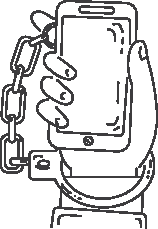
\includegraphics[scale=1.5]{willpower/ch13/3.pdf}
\end{figure}

\subsection*{Сацыяльны ўплыў}

Інтэрнэт ня толькі злучае людзей, якія знаходзяцца далёка адно ад аднаго, але й разьядноўвае тых, хто знаходзіцца побач. Пастаяннае адцягненьне на тэлефон атрымала назву фабінг (phubbing), а~чалавек які адцягваецца завецца~--- фабэр. Фабэр пастаянна перарывае ежу, камунікацыю, паездку на аўтамабілі адцягненьнем на тэлефон. Такія паводзіны разбураюць зносіны, выклікаюць гнеў і раздражненьне суразмоўцы, зьяўляюцца частай прычынай канфліктаў у~сям'і.

Паказана, што людзі без смартфона атрымліваюць прыкметна больш задавальненьня пры камунікацыі. Нават сам факт наяўнасьці тэлефона зьмяншае пачуцьцё блізкасьці і даверу, памяншае эмпатыю і разуменьне партнёра.

\infobox{У лічбавым асяродзьдзі няма паху, смаку, дотыку, эмпатыі~--- і такое беднае асяродзьдзе шкоднае для разьвіцьця. Хочаце шчырай размовы? Выключыце або пакіньце тэлефон у~іншым пакоі~--- гэта просты спосаб паказаць, наколькі важны для вас суразмоўца.}

Лічбавае асяродзьдзе дазваляе шмат экспэрымэнтаваць з~сацыяльнымі ролямі, прымяраць на сябе розныя вобразы, ствараць свой імідж. Але інтэрнэт можа стаць крыніцай ілюзій і толькі раскормліваць эга. Карыстальнікі схільныя фіксавацца на сабе, ствараючы нерэальны вобраз са старанна адабраных і адфоташопленых фатаграфій і аповедаў. Гэта просты і даступны спосаб хутка павысіць сваю самаацэнку, прыцягнуць увагу іншых людзей і сабраць яшчэ больш лайкаў. Па меры павелічэньня канкурэнцыі, людзі гатовыя ісьці на што заўгодна, абы атрымаць дадатковую порцыю віртуальнай сацыяльнай ухвалы. Замест стварэньня чагосьці новага, замест рэальных дзеяньняў, мы спрабуем пераканаць часта нават незнаёмых нам людзей у~сваёй важнасьці, зрабіць на іх уражаньне.

Спробы падняць свой статус анляйн схіляюць да разьвіцьця нарцысічных тэндэнцый. Бо размовы пра сябе так моцна павышаюць узровень дафаміну! Калі ў~асабістай гутарцы мы выказваем сваё меркаваньне толькі 30--40\,\% ад часу гутаркі, то анляйн мы каля 80\,\% часу гаворым толькі пра сябе. Мы не зважаем на невэрбаліку, на інтанацыі, на позірк і да т.~п. Нават нашы рэпосты~--- гэта спосаб зьвярнуць на сябе ўвагу і атрымаць адабрэньне.

\subsection*{Фізычны ўплыў}

Выкарыстаньне смартфона аказвае прыкметны ўплыў на паставу (уключаючы болі ў~шыі і сьпіне, парушэньне крывацёку ў~сасудах шыі і да т.~п.), павялічвае напругу вочных цягліцаў пры сталым разгляданьні блізкіх прадметаў, павялічвае ўзьдзеяньне яркага сьвятла сіняга спэктру (парушэньні сну і біярытмаў~--- падрабязна разабрана ў~разьдзеле ``Сон''), распаўсюджвае электрамагнітнае выпраменьваньне (падрабязна разабрана ў~разьдзеле ``Шкоднае асяродзьдзе''), пагаршае сядзячы лад жыцьця (падрабязна разабрана ў~разьдзеле ``Рух'').

Нерухомасьць правакуе падвышаную рызыку трамбозу, гемарою, бясплодзьдзя (залішні нагрэў яечкаў), спэцыфічныя парушэньні суставаў (артроз вялікага пальца, тунэльны сындром), сындром сухога вока, тэлефон можа быць прычынай траўмаў, калі вы не адрываецеся ад экрана на хаду. Адцягненьне на тэлефон падчас кіраваньня~--- частая прычына аварый і павелічэньне рызыкі загінуць у~ДТЗ.

\infobox{Да 24\,\% усіх аварый выкліканы выкарыстаньнем тэлефона, а~кіроўца са смартфонам эквівалентны п'янаму за рулём. Выкарыстаньне гарнітуры толькі нязначна зьніжае рызыкі.}

Калі мы трымаем тэлефон у~руках, мы глядзім на яго, апусьціўшы галаву ўніз. Куды скіраваны ваш погляд, туды ідзе і галава. А куды зьвернутая галава, туды і ўсе цягліцы цела. Таму калі вы гледзіце ўніз, то вы будзеце горбіцца. З гравітацыяй нашы цягліцы змагаюцца прыгожа, але ж цяпер больш актуальная іншая праблема~--- смартфон. Калі вы гледзіце на экран, то моцна нахіляеце галаву і падымаеце плечы. Гэтую зьяву назвалі «\textbf{тэкставая шыя}» (text neck).

\textbf{Чаму гэта важна?} Чалавечая галава важыць каля 5 кг. Але калі мы нахіляем яе, вага на шыйным аддзеле хрыбта пачынае ўзрастаць. Пад вуглом у~15 градусаў гэтая вага складае каля 12 кіляграмаў, у~30 градусаў~--- 18 кг, у~45 градусаў~--- 22 кг, у~60 градусаў~--- гэта ўжо 27 кг. ``Тэкставая шыя'' прыводзіць да хранічнага запаленьня і наступнай дэфармацыі, зьмяняючы натуральны выгін шыі і ўплываючы на іншыя важныя функцыі, уключаючы кровазабесьпячэньне галаўнога мозгу. Навукоўцы на рэнтгенаўскіх здымках выявілі, што рогападобныя ўтварэньні на задняй паверхні шыі ёсьць у~30\,\% людзей ад 18 да 36 гадоў: чым старэйшы чалавек, тым меншая верагоднасьць наяўнасьці ``рогу''. Такі рог~--- гэта адлюстраваньне фэномэну ``тэкставай шыі'', то бок хранічнай напругі і боляў у~вобласьці галавы і шыі.

\begin{figure}[htb!]
  \centering
  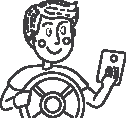
\includegraphics[scale=1.5]{willpower/ch13/4.pdf}\qquad
  
\includegraphics[scale=1.5]{willpower/ch13/5.pdf}
\end{figure}

\emph{Зладзім экспэрымэнт. Прыслухайцеся да тонусу цягліц. Як толькі вы сагняце галаву, то аўтаматычна ўзьнікне павелічэньне тонусу цягліц пярэдняга боку цела і жаданьне сагнуць канцавіны. А калі вы падыміце галаву, то павялічыцца тонус цягліцаў-разгінальнікаў задняй паверхні цела. Паспрабавалі?}

\emph{Цяпер пераходзім да вачэй. Як мы ведаем, глядзець ``зьнізу ўверх'' або ``глядзець звысоку'' не зьвязана з~ростам, а~зьвязана з~напрамкам позірку. Паспрабуйце паглядзець уніз і пры гэтым пачніце адхіляць галаву назад. Адчуваеце супраціў? А зараз падыміце вочы ўгару і пачніце таксама адхіляць галаву назад. Адчуваеце розьніцу?}

\emph{Зараз зрабіце тое ж самае з нахілам наперад: пагляд угару й апускайце плыўна галаву, адчуваеце супраціў? Зараз пагляд уніз і апускайце галаву, адразу ідзе, так? Куды скаваны пагляд, туды ідзе й галава.}

Важна глядзець ``нароўні'', працуючы, сачыць за станам экрана, каб не глядзець уніз. Аптымальны вугал сярэдзіны манітора ад гарызанталі~--- 15 градусаў. Калі вы трымаеце смартфоны унізе, позірк заўсёды будзе ісьці ўніз. Прымусова ўтрымліваць паставу~--- гэта непрацоўная стратэгія. Як толькі вы адцягваецеся, цяглічныя патэрны вяртаюць яе ў~ранейшае становішча. Выснова: ``трэба жыць, не апускаючы вачэй''.

\emph{Сапраўды, як так атрымалася, што раней людзі глядзелі на зоркі ў~тэлескопы, потым апусьцілі позірк у~тэлевізары, а~цяпер нахіляюць галаву, каб глядзець у~смартфон?!}

\subsection*{Спэцыфічныя лічбавыя разлады}

Існуе шэраг спэцыфічных разладаў, зьвязаных з~залішнім знаходжаньнем у~лічбавым асяродзьдзі.

\textbf{Намафобія}~--- страх застацца без тэлефона, цяжкае дыскамфортнае адчуваньне, калі вы без тэлефона. Яе таксама называюць ``лічбавай трывогай''. Існуе анекдот пра тры галоўныя пытаньні сёньня: ``хто вінаваты?'', ``што рабіць?'' і ``дзе мой тэлефон?!''. Частае выкарыстаньне сацыяльных сетак таксама спрыяе ўзмацненьню трывогі, зь іншага боку, больш трывожныя людзі самі па сабе схільныя да мацнейшай залежнасьці ад сацыяльных сетак.

\textbf{Інфадэмія.} Я пішу гэтыя радкі ў~Хуахіне, Тайланд, дзе затрымаўся на няпэўны тэрмін з~прычыны масавай адмены рэйсаў. Прама цяпер мы назіраем нараджэньне тэрміна ``інфадэмія'' (ад пандэмія)~--- наплыў непацверджанай інфармацыі пры адсутнасьці дакладнай інфармацыйнай кампаніі ад дзяржавы і прыманыя ёй хаатычныя меры. Многія людзі сталі ``мэдыяспэкулянтамі'', выказваючы загадзя фальшывыя тэорыі змовы, прапаноўваючы ``вакцыны'' або ``прадукты ад вірусу'', яны танна ``скупляюць увагу'' людзей, якія знаходзяцца ў~стане панікі і трывожнай няпэўнасьці.

\emph{Дасьледаваньні паказваюць, што фэйкавыя навіны атрымліваюць нашмат больш рэпостаў і лайкаў і хутчэй распаўсюджваюцца па сацыяльных сетках, чым дакладная інфармацыя. Яшчэ Эйнштэйн пытаўся: ``Ці магчыма кантраляваць мэнтальную эвалюцыю роду чалавечага такім чынам, каб зрабіць яго ўстойлівым супраць псыхозаў жорсткасьці і разбурэньня?''} 

Інвэстыцыі ў~культуру, адукацыю, выхаваньне ўнутранай сыстэмы каштоўнасьцяў і перакананьняў, самаідэнтычнасьці~--- усё гэта дае надзейны імунітэт супраць псыхічных эпідэміяў. Праўда, сучасныя ўрады, якія абапіраюцца на прапаганду, наўрад ці натхняцца гэтай мэтай. Дасьледаваньні паказваюць, што для зьменаў у~грамадзтве дастаткова толькі 10\,\% упэўненых людзей, таму дзяліцеся карыснай інфармацыяй са сваімі блізкімі і знаёмымі, бо калі мы ня будзем місыянэрамі сваіх ідэй, яны самі па сабе не перамогуць.

\textbf{FOMO (ад анг. fear of missing out)}~--- гэта стан, пры якім чалавеку здаецца, што жыцьцё праходзіць міма яго, што ён прапускае важнае і цікавае, даступнае яго сябрам і знаёмым. Чым больш мы бачым пастоў аб тым, як насычана і ярка жыве наша фрэнд-стужка, тым менш радасным здаецца наша жыцьцё.

\infobox{Амаль 60\,\% карыстачоў нэгатыўна ацэньваюць сваё жыцьцё ў~параўнаньні з~пастамі сваіх сяброў у~сацсетках.} 

Зрэшты, сёньня на замену FOMO прыходзіць абарончая рэакцыі JOMO (joy of missing out), калі вы атрымліваеце задавальненьне, нешта прапусьціўшы, ці калі вы можаце дазволіць сабе нечага ня ведаць і ў~чымсьці ня ўдзельнічаць!

\textbf{«Разумовая сьвярбячка»}~--- гэта дыскамфорт у~стане спакою, калі невыносна хочацца праверыць пошту ці пагартаць навіны, каб пазбавіцца ад гэтага дакучлівага хваравітага жаданьня. Ёсьць яшчэ «Прывідны званок»~--- і гэта ня назва фільма жахаў, а~фантомнае адчуваньне, што ваш тэлефон звоніць. Напрыклад, дарослы амэрыканец правярае тэлефон 40--50 разоў у~дзень, а~ў моладзі гэта значэньне дасягае да 80--90 разоў у~дзень. Пацешна, што шматлікія людзі жудасна баяцца, што іх чыпуюць, але пры гэтым не расстаюцца з~тэлефонам нават у~туалеце.

\emph{Шматзадачнасьць і пастаяннае адцягненьне прыводзіць да «звужэньня гарызонту плянаваньня», людзям становіцца складана складаць пляны на доўгія тэрміны наперад.}

\subsection*{Іншыя праблемныя месцы}

\textbf{Мэдыяскетызм і лічбавая беднасьць.} Калі раней пастаянная прысутнасьць анляйн лічылася гераізмам, то цяпер гэта прыкмета глупства і нястрымнасьці. Дазвольце сабе раскошу адказваць на лісты і паведамленьні тады, калі вам зручна, не апраўдвайцеся, не прасіце прабачэньня, а~для таго, каб пазьбегнуць неразуменьня, выразна пазначце часавыя рамкі, калі вы адказваеце на лісты і чытаеце месэнджэры і пошту. Гэта прывучыць людзей выконваць вашыя ўмовы. Мэдыяскетызм~--- сьвядомае скарачэньне спажываньня кантэнту і анляйн-камунікацыі. Цяпер мы бачым, што лічбавыя тэхналёгіі выціскаюць рэальную камунікацыю, і большасьць людзей вымушаны размаўляць з~тэлефоннымі робатамі. Лічбавая няроўнасьць або лічбавая беднасьць сёньня~--- кансультацыі зь віртуальнымі або анляйн-дактарамі, і навучаньне дзяцей па запісах відэа, без актыўнага ўдзелу выкладчыка.

\infobox{Масавы лічбавы падыход замяняе пэрсанальны падыход жывога чалавека, а~жывая камунікацыя патроху робіцца ўсё даражэйшай.}

\textbf{Смартфон і глябальная нездаволенасьць.} Як прыкмеціў адзін мой сябар, адна з~прычын нарастаньня глябальнай нездаволенасьці~--- гэта паўсюднае выкарыстаньне смартфонаў. Калі раней у~вёсцы ці горадзе багатыя і бедныя жылі кожны ў~сваім сьвеце, то цяпер смартфоны дазваляюць параўноўваць сябе зь людзьмі іншых сацыяльных слаёў. І вельмі часта параўнаньне ідзе не на вашу карысьць. Самаацэнка фармуецца як стаўленьне да сярэдняга ўзроўню людзей вакол вас, а~ў віртуальнай рэальнасьці заўсёды знойдуцца тыя, хто нашмат прыгажэйшы, багацейшы і разумнейшы~--- ну, ці робіць такое ўражаньне.

Мэта рэклямы~--- прымусіць вас адчуць сябе непаўнавартаснымі і кампэнсаваць гэта пакупкай пэўнага тавару. Шчасьлівым спакойным здаровым людзям, якія вызнаюць мінімалізм, складана нешта прадаць. Яны ня будуць галасаваць за сумнеўных палітыкаў, таму іх трэба запалохаць. Выконвайце лічбавую гігіену, яна вельмі патрэбная для яснага розуму і моцнага здароўя.

\textbf{Кібэрбулінг}~--- гэта цкаваньне ў~лічбавай прасторы. І калі прыставаньні ў~школьным двары там жа і сканчаюцца, то кібэрбулінг можа працягвацца бясконца доўга. Беспакаранасьць, ананімнасьць, арганізацыя групы, магчымасьць масавага рассыланьня кампрамэтоўных матэрыялаў, падман,~--- усё гэта правакуе цкаваньне ў~яе розных відах: распаўсюджваньне чутак, абразы, паклёп, пагроза расправы. Кібэрбулінг мае шмат абліччаў: кібэрмобінг, тролінг, флэйм, хэйтынг і таму падобнае, і тычыцца гэта ў~першую чаргу дзяцей.

\emph{Частым зьяўляецца і хэпіслэпінг~--- калі падлеткі зьбіваюць людзей, запісваюць гэта на камэру і выкладваюць у~сеціва.}

У дзяцей няма псыхалягічных рэсурсаў, каб даць рады агрэсіі, і нават адзін абразьлівы камэнтар пад іх фота можа сур'ёзна вывесьці іх зь сябе. З прычыны ананімнасьці кібэрбулінгу і таго, што гэтую інфармацыю бачыць мноства людзей, зьяўляецца адчуваньне бездапаможнасьці. У дзяцей гэта зьніжае пасьпяховасьць, самаацэнку, правакуе да прагулаў, ужываньня алькаголю, прыводзіць да дэпрэсіі і суіцыдаў.

Важна хутка і эфэктыўна дзейнічаць супраць булінгу, не ўступаць у~зносіны з~агрэсарам ні ў~якім выглядзе. Адразу блякуйце булера. Рабіце прынтскрын перапіскі, пры наяўнасьці пагроз або адпраўленьні парнаграфічнага матэрыялу вы маеце права падаць заяву ў~паліцыю, цяпер сеткавая ананімнасьць ужо абсалютна ўмоўная, а~артыкулы, штрафы і тэрміны~--- рэальныя. Зьвяртайцеся ў~службу падтрымкі сацсетак або мэсэнджараў з~патрабаваньнем блякаваць карыстальніка і выдаліць матэрыял, калі справа адбываецца на форуме~--- то да мадэратара тэмы. Калі сацсеткі ці форумы адмаўляюцца дапамагчы, то заява ў~паліцыю можа быць пададзеная і на іх.

Не дазваляйце адзначаць вас на фатаграфіях, не выкладвайце ў~асабістым доступе такія зьвесткі, як нумар тэлефона, паштовы адрас і да т.~п. Прывучыце дзяцей ніколі не выкладваць свае фота і не дзяліцца інфармацыяй пра сябе. Кібэрбулінг часта можа выяўляцца ў~выглядзе сэксуальных правакацый, каб дамагчыся ад вас эратычных фота з~мэтай іх далейшага распаўсюджваньня ці вымагальніцтва. Калі вы відавочца кібэрбулінгу, заўсёды выступайце супраць агрэсара і падтрымлівайце ахвяраў, тым больш што ў~інтэрнэце гэта зрабіць нашмат прасьцей.

Калі раней людзі думалі, што Бог усё бачыць і ведае, то цяпер інтэрнэт усё бачыць, усё ведае і нічога не забывае. Любы тэлефон можа быць узламаны і можна слухаць зь мікрафона, здымаць з~камэры ўсё, што вы робіце і што адбываецца каля вас. Ніколі не размаўляйце па тэлефоне, не адпраўляйце паведамленьні, не пішыце лісты ці не адпраўляйце фота, якія нельга паказаць усяму сьвету.

\textbf{Калі вас нешта закранула, не сьпяшаецеся пісаць гнеўны камэнтар, дайце сабе астыць. Бо ў~інтэрнэце заўсёды нехта будзе ня мець рацыі, і гэта абсалютна нармальна.}

\subsection*{Пытаньні і заданьні}

1. Ці выкарыстоўваеце вы тэлефон падчас камунікацыі зь іншым чалавекам?

2. Як часта вы верылі фэйкавым навінам і пры гэтым адчувалі нэгатыўныя эмоцыі?

3. Ці часта вы адчуваеце незадаволенасьць і зьніжэньне самаацэнкі пасьля выкарыстаньня сацыяльных сетак?


\section{Страта ўвагі. Тонуты мозг}

Франц Кафка неяк заўважыў, што «жыцьцё ўвесь час адцягвае нашую ўвагу; і мы нават не пасьпяваем заўважыць, ад чаго менавіта». Дык вось, лічбавае асяродзьдзе робіць гэта яшчэ больш эфэктыўна. У разьдзеле ``Усьвядомленасьць'' мы з~вамі разабраліся, што ўвага~--- гэта канчатковы рэсурс.

\textbf{Наша ўвага выбарчая: куды мы яе накіроўваем, туды і пераразьмяркоўваюцца рэсурсы мозгу.}

Калі мы пасіўныя, то ўвага аўтаматычна прыцягваецца да ўсіх ``эвалюцыйных трыгераў'': сьмерць або пагроза, сэкс, смачная ежа, павышэньне статусу і іншыя старажытныя праграмы выжываньня. Калі мы ўмеем самі накіроўваць сваю ўвагу, то можам пасьпяхова супраціўляцца адцягвальным чыньнікам ня толькі лічбавага, але й рэальнага сьвету, і выбіраць тое, што нам сапраўды важна і трэба. Адна з~сучасных прычын страты ўвагі~--- гэта павелічэньне інфармацыйнай нагрузкі. У нас эвалюцыйна закладзеная цікаўнасьць, і мозг узнагароджвае нас дафамінам, калі мы даведаемся нешта новае. Мы з~задавальненьнем спажываем інфармацыю, не задумваючыся аб пабочных эфэктах яе лішку. Інфармацыя, як і ежа, уплывае на наш эмацыйны стан і прыманыя рашэньні, нават калі мы гэтага не ўсьведамляем. Гэта ня вы спажываеце інфармацыю, гэта інфармацыя спажывае вашую ўвагу.

\textbf{Інфаатлусьценьне (infobesity)}~--- гэта калі мы распухаем ад лішку інфармацыі, становімся менш здаровымі, таўсьцейшымі і пасіўнымі. Як падлічылі навукоўцы, выпуск The New York Times за тыдзень утрымоўвае больш інфармацыі, чым чалавек XVII стагодзьдзя даведваўся за ўсё жыцьцё. Бо тады навіны распаўсюджваліся праз рэдкія чуткі і аповеды ад купцоў ці вандроўцаў.

Калі вонкавыя стымулы крадуць нашу ўвагу, то ў~нас застаецца менш увагі да сваіх унутраных стымулаў, і нашы паводзіны становіцца рэактыўным (адказваем на вонкавыя стымулы), а~не праактыўным (дзейнічаем па сваім пляне). Трэніроўка ўсьвядомленасьці дапамагае кіраваць сваім фокусам увагі: гледзячы на лужыну, мы можам самі выбіраць, што ў~ёй бачыць~--- бруд ці зоркі.

\infobox{Навык нерэагаваньня дапамагае нам не запускаць асацыятыўную працу розуму, калі мы на нешта глядзім ці атрымліваем новую інфармацыю.}

Існуе \textbf{содневы ліміт інфармацыі}, якую наш мозг можа перастрававаць за дзень бяз шкоды для сябе, і мы павінны сьвядома сачыць за тым, што спажываем у~інфармацыйным асяродзьдзі. Інфармацыя не інэртная~--- яна мяняе нас, таму інфармацыйная гігіена вельмі важная. Неабходна дзейнічаць папераджальна, пазьбягаючы ўзьдзеяньня шкоднай інфармацыі і старанна адбіраючы самае лепшае: не душыцеся інфармацыйным фастфудам на хаду!

\begin{figure}[htb!]
  \centering
  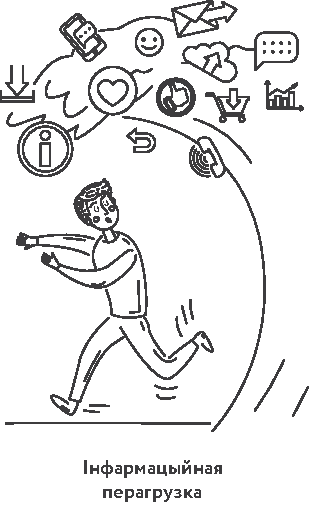
\includegraphics[scale=1.5]{willpower/ch13/6.pdf}
\end{figure}

\emph{«Калі вы павялічваеце працэнт спажываньня агульнадаступнай інфармацыі, вынік вашай разумовай дзейнасьці наўрад ці зможа прэтэндаваць на арыгінальнасьць. Ашалелае імкненьне да стварэньня першапачаткова ёсьць практычна ва ўсіх, проста ў~мяне яно засталося па меры сталеньня і не было выціснутае псэўдакаштошнасьцямі грамадзтва спажываньня. Магчыма, таму што я захоўваў галаву ў~чысьціні: не глядзеў тэлевізар, не чытаў газэтаў, не прымаў на веру меркаваньне аўтарытэтаў». Павел Дураў, стваральнік Вконтакте і Тэлеграм.} 

\textbf{Раскоша выбарчай недасьведчанасьці.} Ня бойцеся прапусьціць нешта сапраўды важнае, так ці інакш вы даведаецеся пра гэта ад навакольных. Спытайце сябе, які адсотак дзённай інфармацыі (навіны, сацсеткі, газеты і інш.) рэальна ўплывае на ўзровень вашага асабістага разьвіцьця і на прыняцьце канкрэтных рашэньняў? Недасьведчанасьць зробіць вас больш спакойнымі, больш шчасьлівымі і больш крэатыўнымі, бо вы не назапашваеце ў~сабе велізарную колькасьць памылак, якія генэруюць самыя розныя аўтары.

\textbf{У наш час назіраецца ўсеагульнае паніжэньне здольнасьці кіраваць сваёй увагай, людзям усё цяжэй засяродзіцца на чымсьці адным на працягу працяглага пэрыяду часу. А бо ў~лічбавы час здольнасьць канцэнтравацца на складаных задачах зьяўляецца самай важнай.}

Пры шматзадачнасьці і сталай стымуляцыі мозгу новымі стымуламі, пераключэньні ўвагі паміж рознымі малюначкамі адбываецца паслабленьне канцэнтрацыі і фармаваньне сымптомаў, якія нагадваюць сындром дэфіцыту ўвагі.

\emph{Нядаўняе дасьледаваньне паказала, што занадта частае карыстаньне смартфонам пагаршае разуменьне навуковых тэкстаў, дзе патрабуецца разуменьне герархіі аргумэнтаў і вялікі аб'ём працоўнай памяці. З дапамогай тамографа ўстаноўлена, што прычына~--- у~памяншэньні актыўнасьці астраўковай долі і ніжняй лобнай зьвіліны галаўнога мозгу, якія адказваюць за канцэнтрацыю і апрацоўку інфармацыі.}

За кожнае асобнае дзеяньне мозг узнагароджвае нас дафамінам, таму нам так падабаецца пераключацца паміж рознымі справамі, рэгулярна правяраць пошту ці колькасьць лайкаў. Але кожнае такое адцягненьне і пераключэньне спажывае вялікую колькасьць энэргіі і ўвагі і аслабляе нашу здольнасьць да працяглай канцэнтрацыі. Шматзадачнасьць аслабляе кагнітыўныя здольнасьці і памяншае шчыльнасьць шэрага рэчыва ў~пасавай кары мозгу, якая адказвае за кантроль эмоцыяў. Нядзіўна, што пры яго аслабленьні чалавеку цяжка стрымліваць свае імпульсы: чым часьцей мы адцягваемся, тым больш слабеюць нэўронавыя сеткі, якія адказваюць за працяглае ўтрыманьне ўвагі.

\textbf{Смартфон~--- свайго роду гульнявы аўтамат}, запраграмаваны на тое, каб увесь час уплываць на чалавека. Падумайце, як часта вы бераце свой тэлефон без канкрэтнай мэты? Гэта як быццам гульня ў~казіно~--- ёсьць лайк ці не, прыйшоў ліст ці не, адказалі на паведамленьне ці не. Такая нявызначанасьць стымулюе выкід дафаміну і яшчэ мацней прывязвае нас да тэлефона. Больш за тое, цяпер і стужку ў~сацсетках немагчыма прагартаць да канца, яна становіцца бясконцай. На відэа-сэрвісах адразу пасьля заканчэньня відэа аўтаматычна ўключаецца наступнае, падабранае пад вашыя густы~--- абы вы не перасталі глядзець. Прымаючы інфармацыю, мы змушаныя адказваць праз сацыяльную ўзаемнасьць: адказваць на лайкі, падпісвацца ў~адказ, адказваць на паведамленьне і да т.~п.

Калі мы не ўсталявалі правілы самі, то вымушаныя падпарадкоўвацца. Якім будзе ваш выбар?

\subsection*{Пытаньні і заданьні}

1. Адцягнуўшыся ад сацыяльных сетак, запішыце, колькі вы правялі там часу, якое ў~вас самаадчуваньне і што карыснага вы даведаліся. Ці вартая гэтая інфармацыя вашага часу?

2. Пачысьціце свае падпіскі. Як вы можаце пазбавіцца ад яшчэ большай колькасьці інфармацыйнага сьмецьця?

3. Каго вы слухаеце ці чытаеце з~блогераў? Хто гэтыя людзі і што яны прадаюць?


\section{Скажэньне рэальнасьці. Жыцьцё ў~лічбавай бурбалцы}

Памятаеце казку, дзе каралева пыталася: «Адкажы, люстэрка, ўміг, хто найпрыгажэй усіх?» Для многіх інтэрнэт стаў такім жа чароўным люстэркам, толькі не такім сумленным і шчырым.

Калі ў~нас няма канкрэтнай мэты, калі мы гуглім або заходзім у~сацыяльную сетку, мы трапляем ва ўладу алгарытмаў. А гэта небясьпечна, бо яны ``ведаюць'', што нам падабаецца і што прымушае нас правесьці ``ў тэлефоне'' яшчэ больш часу. Ключавая задача~--- захапіць найбольшую колькасьць вашай увагі, таму алгарытмы аналізуюць нашы паводзіны і падбіраюць такую інфармацыю, якая кранае нас мацней за ўсё і на якую мы рэагуем ужо аўтаматычна.

\emph{Фатаграфіі людзей, асабліва сяброў, якія паляць ці выпіваюць, правакуюць падлеткаў рабіць тое ж самае. Таму нашы анляйн-сябры і тое, што яны лайкаюць, посьцяць, каментуюць, уплываюць на нас гэтак жа, як і словы рэальных сяброў.}

Калі мы бачым жорсткія камэнтары, навіны ці відэа, гэта робіць і наш мозг больш уразьлівым да стрэсу, зьніжае самаацэнку, мы люстрана ``капіюем'' стрэс. Асабліва таксічныя асобіны або «мэдыяспэкулянты», якія прыцягваюць увагу і сеюць паніку лічбавым клікушствам. Падчас панікі лічбавы дэтокс дапамагае зразумець, што, нават калі вы пабылі бяз сувязі, сьвет жыве і абыходзіцца бяз вашае прысутнасьці анляйн.

\subsection*{Інфармацыйная бурбалка}

Калі мы клікаем на карцінкі ці пасты, алгарытмы гэта запамінаюць і затым, на аснове нашага выбару, фармуюць бурбалку фільтраў. Гэтая бурбалка ўплывае на тое, што мы ўбачым у~сацыяльнай сетцы, тым самым ствараючы моцныя скажэньні.

\emph{Патрапіўшы ў~нейкую анляйн-супольнасьць, карыстальнік можа пачаць лічыць, што паталягічныя дзеяньні~--- нармальныя, бо ў~гэтай групе гэтулькі людзей іх прытрымваюцца!}

Не губляйце сувязі з~рэальнасьцю, не абмяжоўвайце свае зносіны толькі тымі людзьмі, якія цалкам падзяляюць вашыя погляды і думаюць аналягічна. Гэта адно ілюзія ісьціны, таму будзьце падпісаныя і на разумных людзей зь іншымі і нават супрацьлеглымі поглядамі і пазіцыямі, выслухоўвайце іх аргументы і не імкніцеся адпісацца пры найменшых прыкметах дыскамфорту.

\textbf{Адпіска і культура адмены.} У лічбавай прасторы вельмі проста забаніць, адпісацца, заблакаваць ці выдаліць з~сяброў кагосьці~--- гэта нашмат лягчэй, чым сказаць чалавеку нешта ўжывую або абмеркаваць праблему. Таму для многіх становіцца нормай проста прыбіраць са сваёй віртуальнай прасторы нешта, што супярэчыць іх поглядам: унутранае адчуваньне становіцца важнейшым аб'ектыўнай ісьціны.

\textbf{Нягледзячы на дэкляраваную свабоду слова ў~інтэрнэце, карыстальнікі спрабуюць заткнуць, заблакаваць, пагражаць тым, з~кім яны ня згодныя.}

Культура адмены вядзе да таго, што людзі перастаюць выказваць сваё меркаваньне адкрыта, а~абмеркаваньне складаных пытаньняў зводзіцца да прымітыўнай адназначнасьці і нават перасьледу тых, хто думае інакш. Адчуваньне ананімнасьці і беспакаранасьці надае ўпэўненасьць у~сваіх сілах і правакуе людзей на паводзіны, якія яны ня здольныя праявіць твар у~твар.

\emph{Дастаткова згадаць пост Джаан Роўлінг, дзе яна абараняла права жанчынаў называцца жанчынамі, а~не ``людзьмі з~мэнструацыяй'', і агрэсіўную рэакцыю на гэты пост.}

\textbf{Лічбавы сьлед}~--- гэта ўсе нашы дзеяньні ў~інтэрнэце, што мы глядзелі і колькі, што пісалі, каму пісалі. Прыватнасьць тут умоўная: па сутнасьці, усё, што патрапіла ў~інтэрнэт, ніколі з~яго не зьнікне, і нават выдаліць нейкі кантэнт канчаткова~--- гэта вялікая праблема. Апынуўшыся замкнёнымі ў~лічбавай бурбалцы, мы пазбаўляемся магчымасьці ўбачыць альтэрнатыўную інфармацыю. Нават калі мы нешта шукаем у~пошукавіку, выдача падладжваецца не пад адпаведнасьць запыту, а~пад гісторыю нашага пошуку. Атрымліваецца, што мы трапляем у~пятлю, змушаныя круціцца ў~адабранай для нас інфармацыі, штораз замацоўваючы існыя патэрны паводзінаў. 

\infobox{Гісторыя пошукавых запытаў, якая выкарыстоўваецца алгарытмамі, перашкаджае нам зьмяніцца, пашырыць бачаньне сьвету і разумець людзей з~альтэрнатыўнымі поглядамі. Бо мы нават не разумеем, што бачаць іншыя людзі ў~іх выдачы.}

Замыканьне ў~лічбавых бурбалках прыводзіць да радыкалізацыі, сьвет становіцца ўсё больш разьяднаным, узмацняецца пачуцьцё ізаляцыі. Людзі больш нецярпліва ставяцца да носьбітаў супрацьлеглых поглядаў і ўзмацняюць скрайнасьці ў~сваіх поглядах. Бо з~кожным клікам алгарытмы паказваюць вам больш інфармацыі, якая пацьвярджае вашыя погляды, і хаваюць інфармацыю, якая можа прымусіць вас у~іх сумнявацца. Падобны эфэкт атрымаў назву ``культурны трайбалізм'', калі людзі разьбіваюцца на інтэрнэт-плямёны, кожнае зь якіх лічыць свае погляды адзіна правільнымі і пазьбягае ўзаемадзеяньня зь іншымі.

У рэальным сьвеце зьмесьціва кнігі ці кошт тавару не зьмяняюцца ў~залежнасьці ад таго, хто чытае кнігу ці хто купляе тавар. Але ў~лічбавым сьвеце зьмесьціва старонкі і кошт на тавар падладжваюцца пад вас. Факты ператвараюцца ў~ілюзіі, бо першапачатковая мэта алгарытмаў~--- утрымліваць вас як мага даўжэй ля экранаў, паказваючы вам асабістую карціну сьвету, выпінаючы тое, што мацней за ўсё вас прыцягвае або ятрыць. Як можна розным людзям знайсьці агульную мову, калі кожны зь іх бачыць у~экране свайго тэлефона зусім розныя карціны сьвету? Усё гэта адно правакуе і разьдзімае рознагалосьсі.

\subsection*{Лічбавае скажэньне рэальнасьці}

Сацыяльныя сеткі скажаюць рэальнае самаўспрыманьне. Чым больш часу жанчына праводзіць у~сацсетках, чым вышэй для яе важнасьць лайкаў, тым мацней яна схільная да парушэньняў успрыманьня вобразу цела і харчовых паводзінаў. Параўнаньне сябе з~адфаташопленнымі фатаграфіямі мадэляў павышае стрэс і зьніжае самаацэнку.

Адмысловыя фільтры і тэхнічныя хітрыкі (асьвятленьне і вугал здымкі) дазваляюць кожнаму чалавеку здымаць нерэальныя фатаграфіі. Думаю, кожны з~нас дзівіўся, як па-рознаму могуць выглядаць людзі на фота профілю і ў~рэальным жыцьці~--- іх практычна немагчыма пазнаць! Параўноўваючы сябе з~іншымі людзьмі, мы можам пачаць лічыць, што наша жыцьцё нуднае, што мы недастаткова стараемся, што мы няўдалыя ў~параўнаньні з~фэйкавай выдачай у~нашым тэлефоне. Калі прагляд чужых фатаграфій зьніжае самаацэнку, то прагляд сваіх фота і свайго акаўнта павялічвае самаацэнку. \textbf{Таму перагледзець свае шчасьлівыя фатаграфіі~--- гэта выдатная ідэя!}

\textbf{Чаму людзі робяць гэта?} Людзям важна атрымаць сацыяльную ўхвалу, сацыяльнае пацверджаньне, што яны~--- ОК. Калі раней для гэтага трэба было выдатна выглядаць, добра апранацца, выходзіць у~сьвет і зьбіраць кампліменты, то цяпер можна проста рэдагаваць фота і выкладваць іх у~розныя сацсеткі. Нават праграмы для знаёмства патрэбныя ня столькі для сустрэч, колькі для атрыманьня прызнаньня.

\emph{``Зьясі рыбу~--- і будзеш сыты адзін вечар, загуглі рыбу~--- і будзеш бачыць яе цэлы тыдзень'',~--- дзеліцца з~намі сучасная народная мудрасьць. У скажонай рэальнасьці чалавек больш схільны набываць тое, што бачыць на экране, чым актыўна карыстаюцца прадаўцы.}

\subsection*{Пошук нашых уразьлівасьцяў}

Абсалютная большасьць ``бясплатных'' сэрвісаў зусім не бясплатныя. Яны зьбіраюць інфармацыю аб вашых дзеяньнях, аналізуюць яе, знаходзячы вашыя ўпадабаньні. Кожнае ваша дзеяньне ў~інтэрнэце і ў~тэлефоне фіксуецца і захоўвацца, пачынаючы ад таго, колькі секунд вы глядзіце на карцінку, да кожнай вашай пакупкі. З клікаў складаецца поўная карціна вашых паводзінаў, якая дазваляе прадказваць вашыя дзеяньні і рэакцыі. Сутнасьць алгарытмаў~--- гэта ``if it bleeds, it leads'', то бок калі гэта крывавіцца, то будзе прадавацца. Чым мацней у~вас смартфон выклікае эмацыйны водгук, тым больш увагі гэта крадзе і тым даўжэй вы ў~ім седзіце. Чым больш ведаюць пра вас, тым прасьцей выклікаць у~вас рэакцыю, скамбінаваўшы навіны, падкінуўшы пасты людзей, значных для вас, і прапанаваўшы нешта купіць ці зьмяніць меркаваньне.

Доступ да вашых дадзеных можа атрымаць дзяржава, скрасьці хакеры, купіць палітыкі, клінікі, працадаўцы, страхавыя. Выкарыстоўваючы вашыя дадзеныя, можна прымусіць вас купляць нешта, можна прымусіць вас кагосьці ненавідзець, галасаваць патрэбным чынам. Дадзеныя~--- гэта новая нафта. Суровае правіла бясплатнага сыру вястуе: калі вы ня плаціце за выкарыстаньне прадукту, значыць, вы і ёсьць канчатковы прадукт.

\infobox{Памятайце, што ня толькі вы чытаеце артыкул, але і артыкул чытае вас: усё, што вы клікніце, будзе выкарыстана супраць вас.}

Упэўнены, што для сучасных сацыяльных праграмаў павінна быць патрабаваньне рассакрэціць іх алгарытмы і даваць магчымасьць адключыць іх у~асабістым профілі. Але цяпер у~нас нават няма права на прыватнасьць, права адмовіцца ад сачэньня за сабой у~лічбавым асяродзьдзі.

\emph{Дзіўна, але алгарытмы прадказваюць нашыя рашэньні дакладней, чым мы самі. У дасьледаваньнях паказана, што алгарытм дакладней, чым чалавек, прадказвае колькасьць алькаголю, якую вып'е карыстальнік на наступным тыдні, ці за каго прагаласуе.} 

Калі ў~стужцы будзе больш нэгатыву, у~вас пагоршыцца настрой і вы самі станеце пісаць нэгатыўныя пасты. Самае непрыемнае, што няма магчымасьці выключыць гэтую стужку простым спосабам.

\textbf{Сьпіраль маўчаньня.} Нам здаецца, што ў~інтэрнэце мы вольныя, але мы схільныя да ўплыву сваіх падпісчыкаў і сяброў. Людзі неўсьвядомлена імкнуцца пісаць і посьціць тое, што атрымлівае большую колькасьць лайкаў і зьбірае больш ухвалы, а~вось непрыемных тэм пазьбягаюць і не выказваюць думак, якіх не ўхваляе асяродзьдзе. Гэта таксама прыводзіць да скажэньня рэальнасьці і неразуменьня таго, пра што рэальна думаюць людзі. Гэта павялічвае сацыяльны ціск: у~сваёй інфармацыйнай бурбалцы чалавек схільны прымаць гэтыя «навязаныя» погляды як уласныя, каб пазьбегнуць унутранага канфлікту.

У лічбавым асяродзьдзі становіцца складана правяраць праўдзівасьць інфармацыі, асабліва калі ў~нас няма экспэртнасьці ў~тэме. У такім выпадку спрацоўвае статкавы інстынкт і віральнасьць становіцца крытэрам праўдзівасьці~--- чым больш людзей гэта лайкае і дзеліцца, тым быццам бы праўдзівейшая інфармацыя. Чым мацней чапляе ўвагу паведамленьне сваімі эмоцыямі ці абсурдам, тым больш праўдзівым яно здаецца. Масавая пагоня за папулярнасьцю прыводзіць да таго, што велізарная колькасьць людзей спажываюць інфармацыйнае сьмецьце шматкроць на працягу дня~--- а~гэта адбіваецца на псыхічным здароўі не найлепшым чынам.

\textbf{Постпраўда}~--- гэта сытуацыя, калі для фармаваньня пэўнага меркаваньня аб'ектыўныя факты менш важныя, чым эмацыйны камфорт і асабістыя перакананьні. Усё большай колькасьці людзей ісьціна становіцца няважная, а~важна толькі тое, наколькі добра яны сябе адчуваюць. Менавіта таму мы з~задавальненьнем слухаем тых, хто прыемна хлусіць нам, і падманваем самі сябе, выдатна ўсьведамляючы, што ўсё гэта~--- хлусьня.

\textbf{Нарцысізм.} Навукоўцы ўсталявалі, што, чым больш чалавек карыстаецца сацсеткамі, тым ярчэй становіцца выяўленасьць яго нарцысічных рыс, а~ў схільных людзей даходзіць да разьвіцьця нарцысічнага разладу асобы. Паталягічны нарцысізм~--- гэта навязьлівае патрабаваньне любові, зьвязанае з~адсутнасьцю эмпатыі. А адкуль можа ўзяцца эмпатыя да віртуальных суразмоўцаў? Калі вы ня можаце сябе адчуць каштоўным без ухваленьня іншых людзей, вам цяжка вытрымаць крытыку, вы прыніжаеце іншых, каб узьдняць сабе настрой, і ў~вас дакладна ёсьць праблемы з~нарцысізмам.

\emph{Першае сэлфі было зроблена ў~1839 годзе, а~цяпер гэта стала паўсюдным сродкам самапрэзэнтацыі. Выяўляем сябе такімі, якімі хочам сябе бачыць і якімі спадабаемся іншым, каб сабраць лайкі. Вядома, акрамя прэзэнтацыі гэта яшчэ адна спроба зьвярнуць на сябе ўвагу, падняць самаацэнку. І далёка не заўсёды бясьпечная~--- спрабуючы прыцягнуць увагу незвычайным сэлфі, людзі гінуць.} 

\infobox{Ад сэлфі гіне больш людзей, чым ад нападу акул.}

У анляйн-размовах мы не атрымліваем зваротнай сувязі ад суразмоўцаў, але атрымліваем шмат дафаміну, прэзэнтуючы сябе і любуючыся сабой. Нашы анляйн-старонкі становяцца для нас крыніцай самаідэнтыфікацыі, а~іх прагляд падвышае самаацэнку. Зьвяртаючыся да групы людзей, мы схільныя перабольшваць рэчаіснасьць у~параўнаньні з~асабістай размовай з~адным чалавекам.

\emph{Мяняецца нават маўленьне: словы ``мы'' і ``даваць'' цяпер выкарыстоўваюць прыкметна радзей, а~``я'' і ``атрымліваць''~--- часьцей.}

\subsection*{Пытаньні і заданьні}

1. Ці часта вы купляеце тавары, якія рэклямуюцца ў~інтэрнэце? Чым вас чапляе іх рэкляма?

2. Ці выкладваеце вы шмат асабістай інфармацыі пра сябе ў~сетку?

3. Ці ёсьць у~вас сябры і ці падпісаныя вы на тых, з~чыім меркаваньнем ня згодныя?


\section{Навіновае порна, лічбавае порна, фуд-порна і іншыя}

Сапраўдныя рыбалоўныя гаплікі для мозгу~--- гэта ўсё, што зьвязана з~размнажэньнем і выжываньнем. Калі гаворка ідзе пра грошы, ежу, сэкс, уладу, сьмерць, катастрофы, бясплатныя паслугі, спосабы хутка стаць знакамітым і багатым, то гэтым вельмі лёгка прыцягнуць увагу. Гіпертрафаваная фіксацыя на гэтым, што ігнаруе мэтазгоднасьць і рэалістычнасьць, часам завецца порна.

Лічбавыя тэхналёгіі дазваляюць эксплюатаваць чалавечую біялёгію ў~вялікіх маштабах і нашмат мацней, чым аналягавыя спосабы. Любая залішняя стымуляцыя прыводзіць да зьніжэньня адчувальнасьці, да страты смаку да жыцьця. Па ступені стымуляцыі дафамінавых рэцэптараў навіновыя парталы шкодзяць нашмат мацней за суседзкія плёткі, лічбавае порна~--- нашмат мацней за порначасопіс. Звычайнае абжорства з~дапамогай лічбавых тэхналёгіяў можна ператварыць у~фуд-порна, а~імпульсіўныя пакупкі~--- у~порна-шопінг, а~палітычныя дэбаты~--- проста ў~клаўнаду. Зразумела, порна ня мае нічога агульнага з~сэксам, толькі эксплюатуе біялёгію, узьдзейнічаючы разбуральна: людзі, якія глядзяць порна, рэдка займаюцца сэксам. Нявінныя быццам бы забавы могуць мець дастаткова сур'ёзныя наступствы для нашага здароўя і самаадчуваньня.

\emph{Ёсьць анекдот: муж пытаецца ў~жонкі: «Чаму ты ўвесь час глядзіш кулінарныя кнігі, але нічога не гатуеш?~--- Ты таксама ўвесь час глядзіш порна, і таксама нічога не адбываецца».}

\begin{figure*}[htb!]
  \centering
  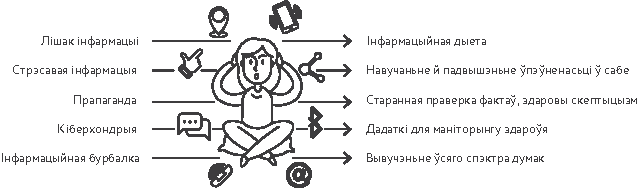
\includegraphics[scale=1.5]{willpower/ch13/7.pdf}
\end{figure*}

\textbf{Фуд-порна}~--- здымка ежы буйным плянам, фота ці відэа, са спэцыяльнымі эфэктамі, з~мэтай выклікаць узбуджэньне ў~чалавека. Навукова даведзена, што выявы ежы вельмі моцна ўзьдзейнічаюць на нашу фізыялёгію і актыўнасьць мозгу: разгляданьне малюнкаў можа выклікаць голад і жаданьне есьці ў~цалкам сытага здаровага чалавека. Фуд-порна~--- гэта калі важная не карысьць, смак ці склад, а~менавіта прывабнасьць, апэтытнасьць. Такія гіпэррэалітычныя кадры, яркія і агрэсіўныя, прыцягваюць нашу ўвагу і стымулююць апэтыт.

\emph{Цікава, што рост папулярнасьці фота ежы і кулінарных шоў прапарцыйны зьніжэньню часу гатаваньня і павелічэньню ўжываньня паўфабрыкатаў.}

\textbf{Лічбавае порна}~--- гэта магутная стымуляцыя дафамінавых рэцэптараў, якая прыводзіць да доўгатэрміновага зьніжэньня тэстастэрону, матывацыі і да выгараньня. Дафамінавая «халява» вельмі небясьпечная для падтрыманьня ўзроўню энэргіі. Небясьпека ж менавіта лічбавага порна ў~тым, што яно ўвесь час прапануе навізну, правакуе павышаць узровень жорсткасьці і не дае ніякага рэальнага досьведу. 

\infobox{Прыбярыце порна і стымуляцыю са свайго жыцьця, і вы адчуеце павышэньне лібіда і смаку жыцьця.}

\textbf{Порна-палітыка.} Гэта дэфармаваньне сучаснай палітычнай сыстэмы, разбурэньне інстытуту рэпутацыі, калі залогам папулярнасьці зьяўляецца паясьнічаньне, хлусьня, пагрозы, абсурдныя заявы~--- усё толькі для таго, каб скрасьці больш увагі гледачоў. Сэнсавая нагрузка палітычных прамоваў пры гэтым імкнецца да нуля. Калі вы абураецеся і адцягваецеся ад працы~--- гэта спрацавала!

\textbf{Навіны.} Нам так прыемна быць у~курсе таго, што адбываецца, што мы нават не разумеем прыхаванай небясьпекі такіх паводзінаў. Навіны~--- гэта чысты цукар для нашага розуму, іх можна спажываць бясконца. Навіны павышаюць узровень дафаміну, не выпадкова многія пачынаюць дзень з~набору стымулятараў: цукар, кафэін і стужка навінаў. Навіны даюцца нам маленькімі кавалачкамі, іх лёгка чытаць, гэта не патрабуе ніякіх намаганьняў, але стварае прыемнае ўражаньне дасьведчанасьці, таму спажываньне навінаў можа выклікаць самую сапраўдную залежнасьць. Гэта амаль заўсёды нэгатыў: у~экспэрымэнтах удзельнікі часьцей чыталі менавіта нэгатыўныя навіны, а~не нэўтральныя ці пазітыўныя. Гэтую нашу асаблівасьць мэдыя эксплюатуюць увесь час: 95\,\% навінаў~--- гэта плёткі, забойствы, сьмерці, трагедыі, катастрофы, крызісы, праблемы і пакуты іншых людзей.

\emph{Нельга сказаць, што таксічныя навіны~--- гэта вынаходства апошняга часу. Ужо ў~1927 годзе траціну плошчы брытанскіх таблёідаў займала інфармацыя аб злачынствах, а~астатняе~--- чуткі, спорт, палітыка. Гэта чытво для мігдаліны, а~не прэфрантальнай кары. Мозг прагне гэтага, каб запазычыць з~такога аповеду нешта карыснае для выжываньня. Насамрэч мы нічога карыснага асабіста для сябе не атрымліваем, а~толькі ўзмацняем стрэс і марнуем ўвагу. Калі мы чытаем пра падзеі, на якія ня можам паўплываць, гэта схіляе да бездапаможнасьці. Навіны прапануюць спрошчанае тлумачэньне падзей і правакуюць кагнітыўныя памылкі, прыгнятаюць творчасьць, стымулююць пракрастынацыю і, на жаль, не даюць намі ніякай карыснай для дзеяў інфармацыі.}

Навіны часта пішуць журналісты, якія выкарыстоўваюць цяжкі арсэнал мэтадаў прапаганды, так пад соўсам навін мы атрымліваем прамываньне мазгоў. Частае паўтарэньне аднаго і таго ж, напрыклад, прыводзіць да таго, што мы пачынаем гэтаму верыць. Такія навіны ніколі не асьвятляюць дэталі, а~толькі даюць адзнакі і начэпліваюць цэтлікі. Адпісвайцеся ад тых, хто рэпосьціць дрэнныя навіны, менш камунікуйце з~тымі, хто ўвесь час залівае ваш мозг крывавымі і халодна-страшэннымі гісторыямі. Нэгатыўная інфармацыя нашмат хутчэй апрацоўваецца мозгам і дае цялесную рэакцыю ў~выглядзе павышэньня актыўнасьці сімпатыйнай стрэсавай сыстэмы. Калі гэта паўтараецца штодня, то можа прывесьці да выгараньня, дэпрэсіі, трывогі~--- мы пачынаем глядзець на сьвет празь несьвядомыя фільтры недаверу і трывогі.

\infobox{Чытаючы навіны, задавайце сабе пытаньне, ці датычыцца гэта асабіста вас? Калі не, дык не спажывайце гэтую інфармацыю і беражыце сваю энэргію.}

Інфармацыя павінна стымуляваць да дзеяньня, а~не фармаваць пасіўнасьць. Звузьце фокус увагі да навін вашага раёна і мястэчка, дзе вы можаце прыняць удзел у~фармаваньні рэчаіснасьці і паўплываць на жыцьцё сваё і асяродзьдзя. Выберыце сабе кола сяброў і лепш цікаўцеся навінамі ў~іх. Таксама можна плаціць за кантэнт правераным выданьням, хто не зарабляе на рэкляме.

\textbf{Ня бойцеся быць ня ў~курсе}~--- гэта ваша канкурэнтная перавага ў~сучасным лічбавым сьвеце. Даведвацца навіны ад паважанага вамі калегі нашмат бясьпечней для псыхічнага здароўя, чым з~тэлевізара. Чытаньне кніг, камунікацыя, спэцыялізаваныя прафэсійныя выданьні карыснейшыя за навіновае сьмецьце. Мэта мэдыяў у~тым, каб любую праблему зрабіць тваёй асабістай праблемай. Ці трэба вам гэта?

\emph{Адмоўцеся праглынаць тое сьмецьце, якое запіхвае ў~вас СМІ, гэта толькі таннае тлумачэньне таго, што адбываецца, ня мае нічога агульнага з~рэальнасьцю. Хочаце ў~гэтым пераканацца? Знайдзіце падшыўку газэтаў дзесяці- або дваццацігадовай даўнасьці і пачытайце навіны. Вы зразумееце, што яны бескарысныя для прыняцьця рашэньняў.}

\textbf{Фэйкі.} Навіны крадуць ня толькі вашу ўвагу, але й час, вы губляеце канцэнтрацыю і каштоўныя рэсурсы. У навінах цяпер практычна немагчыма ўбачыць экспэртаў з~рэпутацыяй, а~ёсьць толькі ``зоркі'', чыя сумнеўная слава аказваецца важнейшая, чым праўдзівасьць інфармацыі. На жаль, цяпер нават сур'ёзныя журналісты ўсё часьцей не праводзяць праверку фактаў і выкарыстоўваюць прапаганду, працуючы на сваіх гаспадароў. Зразумець хлусьню ў~анляйне нашмат складаней, чым пры асабістай сустрэчы, таму лічбавай прапагандзе так проста нас падмануць.

\subsection*{Пытаньні і заданьні}

1. Прыбярыце ўсе крыніцы навін на тыдзень. Не глядзіце тэлевізар, не дакранайцеся да газэты. Спадабалася? Зрабіце гэта сталай звычкай. А калі нешта цікава, то лепш спытайце ў~сяброў~--- будзе і тэма для размовы.

2. Устрымлівайцеся ад розных відаў лічбавага порна: фуд-порна, хэйт-порна, віктым-порна, порна-палітыкі і да т.~п.

3. Даведайцеся навіны вашага раёна, ужывую пагаварыце з~суседзямі і сябрамі.


\section{Тэхніка бясьпекі}

«Я думаю, такім чынам, я існую»~--- казалі старажытныя. Сёньня мы кажам: «Я думаю, такім чынам, у~мяне разрадзіўся смартфон». Вядома, як і было напісана ў~пачатку гэтага разьдзела, лічбавыя тэхналёгіі~--- неад'емная частка нашага жыцьця, і мы ня зможам бязь іх абысьціся. Важна быць прасунутымі і актыўна вывучаць, як можна выкарыстоўваць новыя лічбавыя магчымасьці для павышэньня якасьці жыцьця. Але ў~пагоні за перавагамі важна выконваць тэхніку бясьпекі. Хачу прапанаваць вам набор ідэяў і парадаў~--- вы можаце абраць зь іх тое, што будзе лепш за ўсё працаваць менавіта для вас.

\subsection*{Межы і буфэры}

Усталюйце канкрэтныя межы выкарыстаньня смартфона. Гэта можа быць колькасьць гадзінаў для сацсетак, чытаньня, зносін або фізычныя межы, напрыклад, забарона на выкарыстаньне тэлефона ў~спальні і на кухні. Падумайце, куды вы можаце схадзіць без тэлефона? Пастрыгчыся, пагуляць у~парку, адправіцца ў~краму? Павялічвайце колькасьць такіх ``чыстых'' часавых зон, калі ў~вас побач няма тэлефона. Калі тэлефон неабходны як камера, уключыце авіярэжым. Ніколі і ні пры якіх абставінах не бярыце тэлефон у~ложак~--- гэта вельмі шкодная звычка, якая замінае паўнавартаснаму сну.

\infobox{Самыя эфэктыўныя~--- раніца да 12:00 і вечар пасьля 20:00 без сацыяльных сетак. Вызначце месцы, куды ня будзеце браць тэлефон ніколі, напрыклад лазенка, прыбіральня, кухня, спальня. Калі баіцеся праспаць, купіце звычайны будзільнік, а~не пачынайце свой дзень, хапаючы тэлефон і на аўтамаце пачынаючы яго праглядаць.}

Для адсочваньня межаў усталюйце праграмы, якія паказваюць, колькі разоў вы карысталіся тэлефонам і чым менавіта. Вы можаце ўсталяваць содневыя ліміты для кожнае праграмы. Адсочвайце агульны час, праведзены ў~смартфоне,~--- гэтыя лічбы могуць вас жахнуць, асабліва калі вы падлічыце выдаткаваны за год час.

\emph{Навукоўцы ўстанавілі, што людзі выкарыстоўваюць тэлефон на 11\,\% часьцей толькі таму, што той ляжыць у~іх пад рукой.}

Не бярыце ў~рукі тэлефон, калі размаўляеце з~блізкімі і сябрамі,~--- гэта тэлефонны этыкет.

\textbf{Сацыяльныя сеткі.} Сацыяльныя сеткі дапамагаюць нам падтрымліваць вялікую колькасьць сацыяльных сувязей, мець зносіны з~важнымі для нас людзьмі. Навукоўцы адзначылі, што для павышэньня ўзроўню шчасьця чалавеку трэба атрымаць 60 цёплых камэнтароў у~месяц, таму і самі ня сквапцеся на кампліменты. Адпішыцеся ад тых, хто крадзе вашу ўвагу і час, пакіньце сяброў, якія даюць якасны кантэнт, карысны для прыняцьця рашэньняў і ўвасабленьня іх у~жыцьцё.

\begin{figure}[htb!]
  \centering
  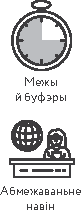
\includegraphics[scale=1.5]{willpower/ch13/8.pdf}\qquad
  
\includegraphics[scale=1.5]{willpower/ch13/9.pdf}
\end{figure}

Пакідайце разгорнутыя камэнтары да цікавых для вас тэмаў, узаемадзейнічайце з~аднадумцамі. Ніколі не выказвайцеся рэзка, нікога не крытыкуйце, нават у~асабістых паведамленьнях. Памятайце, што ўсё напісанае і сказанае можа стаць публічным, таму выконвайце лічбавую бясьпеку. Не захоўвайце важныя дакументы, дадзеныя карт, інтымныя фота ў~ненадзейных агульнадаступных сховішчах дадзеных. Не публікуйце асабістую інфармацыю~--- гэта можа быць выкарыстана супраць вас.

\textbf{Мэтанакіраванае выкарыстаньне.} Смартфон~--- гэта ``соска для дарослых'', так жартуюць дзеці. Навучыцеся адрозьніваць, калі вы бераце тэлефон для вырашэньня канкрэтнай задачы, а~калі ад нуды. «Што я зараз зьбіраюся рабіць і колькі часу на гэта патрачу?»~--- пытайце і адказвайце шчыра. Калі ваш адказ ``нуда'' ці ``стрэс'', то знаходзьце больш здаровыя забаўкі і спосабы для зьніжэньня стрэсу. Прыцягвайце да лічбавага дэтоксу і сяброў, напрыклад, дамоўцеся пры сустрэчы скласьці ўсе тэлефоны ў~адну скрынку на стале.

\subsection*{Лічбавае ўпарадкаваньне}

Ня буду заклікаць вас выкінуць смартфон і купіць тэлефон-раскладушку, але добра б мець простыя спосабы сувязі накшталт кнопкавага тэлефона ці бранзалета-гадзіньніка зь сімкай. Выдаліце лішнія праграмы, адпішыцеся ад непатрэбных старонак і паштовых рассылак~--- зладзьце вялікую прыборку! Выдаліце ўсе апавяшчэньні ад праграмаў, акрамя крытычна важных.

Многія людзі пачынаюць парадкаваць свой лічбавы сьвет з~крайнасьцяў, выдаляючы практычна ўсё,~--- і прайграюць. Прыбірайце сваю лічбавую прастору паводле мэтаду Конда: яна раіць прыбіраць з~дому тыя рэчы, якія не прыносяць радасьці. Пакіньце ў~сваёй лічбавай прасторы толькі тое, што важна, і прыбярыце ўсё астатняе. Калі ня ўпэўненыя~--- выдаляйце. Лічбавае сьмецьце мае сваю цану, яно крадзе вашу ўвагу і час на тое, што сапраўды важна для вас. Замест укараненьня дадатковых абмежаваньняў проста прыбірайце лішняе, ня толькі праграмы, але і дэвайсы. Пытайце сябе~--- эканомяць яны ваш час або марнуюць?

\textbf{Ускладніце доступ}~--- напрыклад, увядзіце ручны набор доўгага пароля да праграмаў, стварыце тэчкі для праграмаў і схавайце іх далей. Разьмяжуйце месэнджэры для дома і для працы. Напрыклад, у~адным мэсэнджэры вы можаце чытаць падпіскі, працаваць у~другім, мець зносіны зь сябрамі ў~трэцім. Па такім жа прынцыпе вы можаце выкарыстоўваць розныя браўзэры як у~смартфоне, так і на хатнім кампутары. Калі ў~вас прафэсійная неабходнасьць быць у~шматлікіх мэсэнджарах ці сацсетках, завядзіце для іх асобны смартфон, які ня трэба заўсёды і ўсюды браць з~сабой.

Адключыце ўсе апавяшчэньні ад праграмаў, акрамя канала сувязі з~блізкімі. Для зьніжэньня візуальнай нагрузкі вы можаце выкарыстоўваць пастаянны рэжым ``вячэрняга экрана'' або чорна-белы рэжым для меншага адцягненьня, самы радыкальны спосаб~--- гэта e-ink экраны, якія не выпраменьваюць сьвятло, яны прыцягваюць увагу менш за ўсё. Няхай ваша застаўка на тэлефоне будзе пустым фонам з~пытаньнем, якое павышае вашу прадуктыўнасьць, напрыклад: «Што я зараз зьбіраюся рабіць?», «Навошта я ўзяў тэлефон?», «Што мне зараз трэба?»

\begin{figure}[htb!]
  \centering
  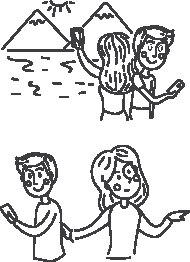
\includegraphics[scale=1.5]{willpower/ch13/10.pdf}\bigskip

  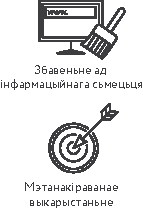
\includegraphics[scale=1.5]{willpower/ch13/11.pdf}
\end{figure}

\infobox{Вядома, ад тэхналёгіяў ня трэба адмаўляцца, нам трэба ўпарадкаваць нашы адносіны з~тэлефонам.}

Тэлефон~--- гэта інструмэнт. А добры інструмэнт~--- той, якім мы карыстаемся для вырашэньня якога-небудзь пытаньня, а~потым адкладаем яго ўбок і займаецца сваімі справамі. Вы павінны кіраваць тэлефонам, а~ня ён~--- выкарыстоўваць вас. Але тэлефон жа адцягвае нас увесь час. Сёньня мы трацім на яго ў~сярэднім дзьве з~паловай гадзіны свайго жыцьця.

Ухіліце тое, чым ён вас чапляе: гук і вібрацыі (уключыце бясшумны рэжым). Прыбярыце тэлефон з~поля зроку (пакладзіце за ноўтбук або ў~шуфлядку). Выкарыстоўвайце іншыя прылады, каб лішні раз ня браць яго ў~рукі. Так, я зноў нашу гадзіньнік на руцэ, так я магу даведацца час, не дастаючы тэлефон. Або выкарыстоўваю асобны таймэр, каб кантраляваць свой графік працы, а~таксама чытаю з~рыдара, а~не экрана тэлефона.

\textbf{Разьбярыце лічбавае сьмецьце}: ачысьціце пошту, адпішыцеся ад абнаўленьняў і супольнасьцяў, усталюйце спэцыяльныя плагіны, якія блакуюць усё, акрамя галоўнай функцыі, напрыклад News Feed Eradicator для адключэньня стужкі фэйсбука, блакавальнікі рэклямы і рэкамэндаваных відэа, напрыклад No Distractions для ютуба. Чым чысьцейшае ваша візуальнае поле, тым прасьцей засяродзіцца. Кожная лічбавая прастора, няхай гэта будзе праграма або сайт, гэта пастка, спраектаваная разумнымі людзьмі, каб завалодаць вашай увагай. Чым часьцей вы карыстаецеся імі, тым горш кіруеце сваёй увагай.

\emph{Усталюйце праграмы для дыхальных практык, для мэдытацыі, для хуткіх нататак, разнастайныя таймэры, якія ня будуць даваць вам ``заліпаць''. Усталюйце праграмы для блакаваньня рэклямы. Карыснымі будуць і пошукавікі накшталт DuckDuckGo, якія выдаюць непэрсаналізаваную выдачу.}

\textbf{Выкарыстоўвайце аналягавыя мэтады.} Часьцей чытайце папяровыя кнігі, пішыце канспэкты, карыстайцеся папяровым дзёньнікам. Дасьледаваньні паказалі, што запіс канспэкта ад рукі больш эфэктыўны для разуменьня і запамінаньня матэрыялу, чым набор на ноўтбуку.

\subsection*{Кібэрхондрыя}

Акрамя розных відаў псэўда-дыягностыкі трывог людзям дадае і самодыягностікі. Інтэрнэт дазваляе зрабіць гэта нашмат больш эфэктыўна, чым стары добры даведнік хваробаў. Уласна, для такой зьявы ёсьць і асобны тэрмін кіберхондрыі~--- гэта імкненьне ставіць сабе дыягназы на падставе сымптомаў, знойдзеных у~пошукавіку.

\emph{«Чаму ты такі сумны?~--- У мяне сындром сумных наднырачнікаў.~--- А дзе падхапіў? -- Выпадкова зайшоў у~адну суполку ў~Facebook».} 

Чаму ж гэта дрэнна, бо інфармацыя пра сябе~--- гэта так карысна!? Уся справа ў~скажэньні рэальнасьці: людзі схільныя шукаць «аднадумцаў» з~падобнымі сымптомамі і прыпісваць сабе іх захворваньні і лячэньне, амаль 50\,\% упэўненыя ў~тым дыягназе, які самі сабе паставілі~--- у~рэальнасьці слушныя менш за 15\,\% самадыягназаў.

\emph{Дасьледаваньне паказала, што 80\,\% карыстачоў гугляць сымптомы, пры гэтым 75\,\% зь іх не правяраюць крыніцу дадзеных і прыналежнасьць сайта.}

Большасьць карыстальнікаў робяць выснову аб дакладнасьці сайта на аснове яго дызайну, простасьці пошуку ў~ім і зразумелага апісання~--- гэтага цалкам дастаткова, каб пачаць давяраць. 75\,\% людзей зважаюць і на іншыя дыягназы, якія ёсць у~выдачы ці апісаннях. А калі гугліць часта, то можна апынуцца ў~бурбалцы фільтраў, калі чалавеку адусюль лезе рэклама лячэння, сімптомы хвароб і гісторыі ``выжылых''.

\infobox{Наш мозг мае і кагнітыўную памылку: чым больш мы даведаемся пра хваробу, тым больш верагоднай яна нам здаецца.}

Чым гэта кепска? Трывожныя разлады пагаршаюць якасьць жыцьця, павялічваюць верагоднасьць ятрагеніі. Калі чалавек няправільна тлумачыць свае сымптомы, гэта можа прывесьці да пагаршэньня недыягнаставанага захворваньня: чалавек праводзіць час, накручваючы сябе і зьніжаючы настрой, замест таго, каб заняцца справай. 

\textbf{Прыкметамі кіберхондрыі зьяўляюцца:} 
\begin{itemize}
  \item занадта частае выкарыстаньне інтэрнэту для пошуку інфармацыі аб сваіх праблемах;
  \item захапленьне анляйн-аб\-сьле\-да\-вань\-ня\-мі;
  \item частая зьмена лекараў;
  \item упэўненасьць у~тым, што ў~здаровага ня можа быць ніякіх прыкметаў захворваньняў;
  \item чытаньне спэцыялізаваных мэдыцынскіх сайтаў;
  \item выбар найбольш цяжкай хваробы з~магчымых.
\end{itemize}

Кіберхондрык з~падазрэньнем ставіцца да мэдыцыны: ``не такі страшны паразіт, як паразітафоб''~--- кажа народная мудрасьць. Калі вы заўважылі, што пошук сымптомаў становіцца навязьлівым, а~сам працэс пошуку і чытаньня прыводзіць да пагаршэньня сымптомаў і настрою~--- гэта нагода для турботы. А наколькі вы схільныя да кіберхондрыі?

\subsection*{Пытаньні і заданьні}

1. Вымярайце час, якое праводзіцца ў~смартфоне, усталяваўшы спэцыяльныя праграмы, напрыклад, Screen time. Вы можаце ўсталяваць асобныя абмежаваньні для кожнай праграмы.

2. Дзякуйце і хваліце ў~анляйне, гэта карысна і вам, і таму, каму вы дзякуеце.

3. Практыкуйце як мінімум раз на тыдзень лічбавы дэтокс. Памятайце, што «сапраўднае жыцьцё~--- гэта тое, што адбываецца, пакуль ваш тэлефон выключаны».

\clearpage
\thispagestyle{empty}
\begin{figure*}[htb!]
  \vspace*{-0.25in}
  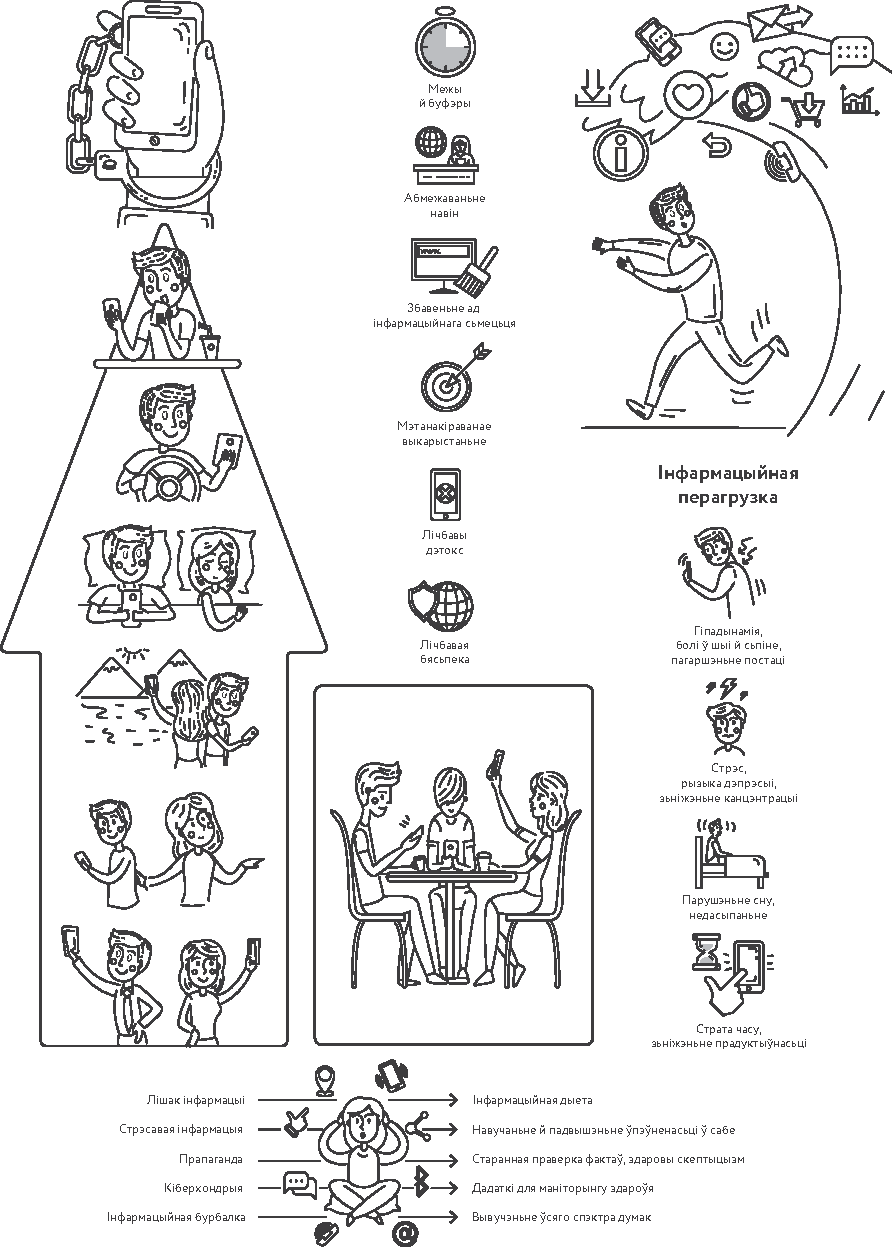
\includegraphics[width=\textwidth]{willpower/ch13/full.pdf}  
\end{figure*}
